%DO NOT MESS AROUND WITH THE CODE ON THIS PAGE UNLESS YOU %REALLY KNOW WHAT YOU ARE DOING

\chapter{Exercises with Matlab}


\section{ Mean value, variance and standard deviation } \label{ Mean value, variance and standard deviation} 
\lstset{language=Matlab,%
    %basicstyle=\color{red},
    basicstyle=\scriptsize,
    breaklines=true,%
    morekeywords={matlab2tikz},
    keywordstyle=\color{blue},%
    morekeywords=[2]{1}, keywordstyle=[2]{\color{black}},
    identifierstyle=\color{black},%
    stringstyle=\color{mylilas},
    commentstyle=\color{mygreen},%
    showstringspaces=false,%without this there will be a symbol in the places where there is a space
    emph=[1]{for,end,break},emphstyle=[1]\color{red}, %some words to emphasise
    %emph=[2]{word1,word2}, emphstyle=[2]{style},    
}
\noindent \textbf{Task:} Generate 1000 on the interval [0, 1] uniformly distributed random numbers. Display the numbers by using the MATLAB-instruction \texttt{plot.} Before generating the random numbers the initial value has to be set to 0 via the option \texttt{state} in the MATLAB function \texttt{rand}. Save the vector of random numbers in \texttt{dat1\_1}. Calculate the mean value, variance and standard deviation of the random sequence in three different ways.
\newline
\noindent Using the MATLAB
\begin{enumerate}
\item loop \texttt{for ... end},
\item functions \texttt{sum} and \texttt{length} and
\item functions \texttt{mean} and \texttt{cov}.
\end{enumerate}
Compare the results. Take a look at the m-files \texttt{mean} and \texttt{cov} with the instruction type. 
\noindent \textbf{Solution:}
\noindent We can create 1000 uniformly distributed random numbers by using the function \texttt{rand}. We have written separate functions in-order to have a clean code. First, the function \texttt{randomSequence} is written to generate uniformly distributed random numbers, then three separate functions called to calculate the mean value, variance and standard deviation in the mentioned ways. Lastly, the \texttt{compare} function aids to compare the result.

\noindent \textbf{MATLAB code:}
\lstinputlisting{assignment1_1.m}

\noindent \textbf{Output:}
\noindent The plot of uniformly distributed random numbers over the interval [0,1] is depicted in Figure 2.1.
\begin{figure}[H]
\centering
{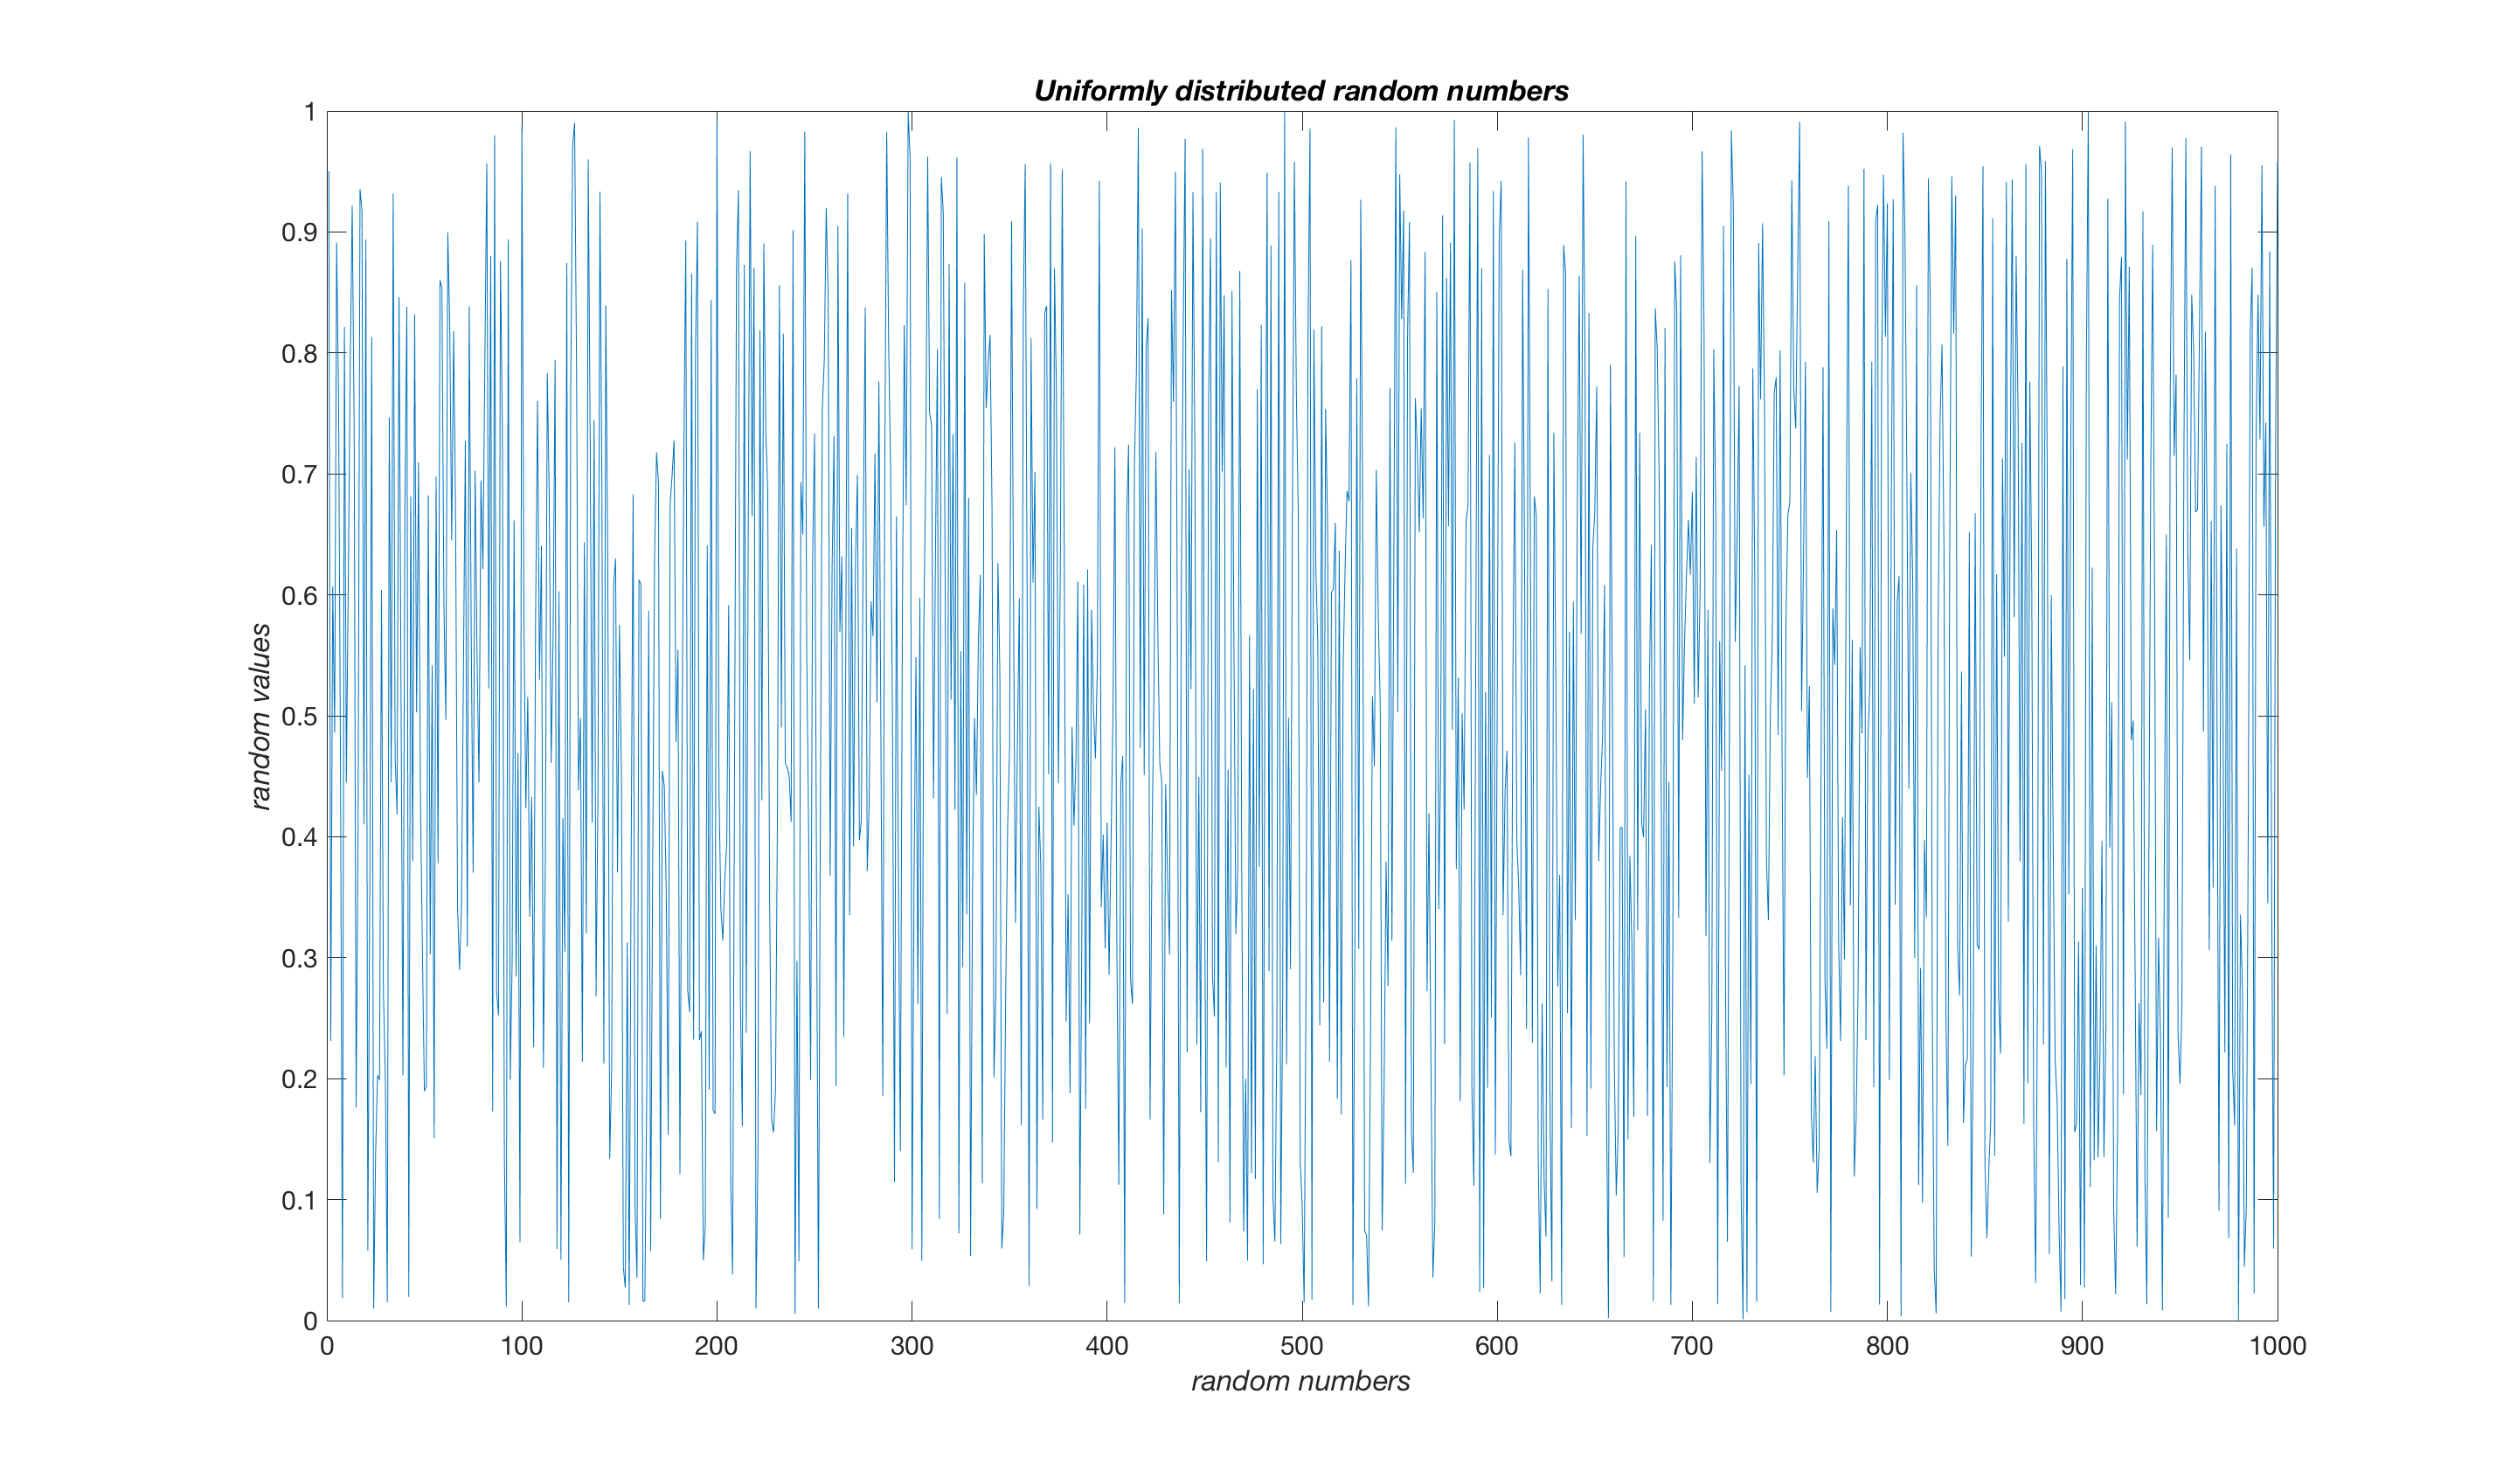
\includegraphics[scale=0.12]{ass1_1.png}}
\caption{Uniformly distributed random variables in the interval [0,1]}
\end{figure}
\noindent The output of the code is shown below.
\begin{figure}[H]
\centering
{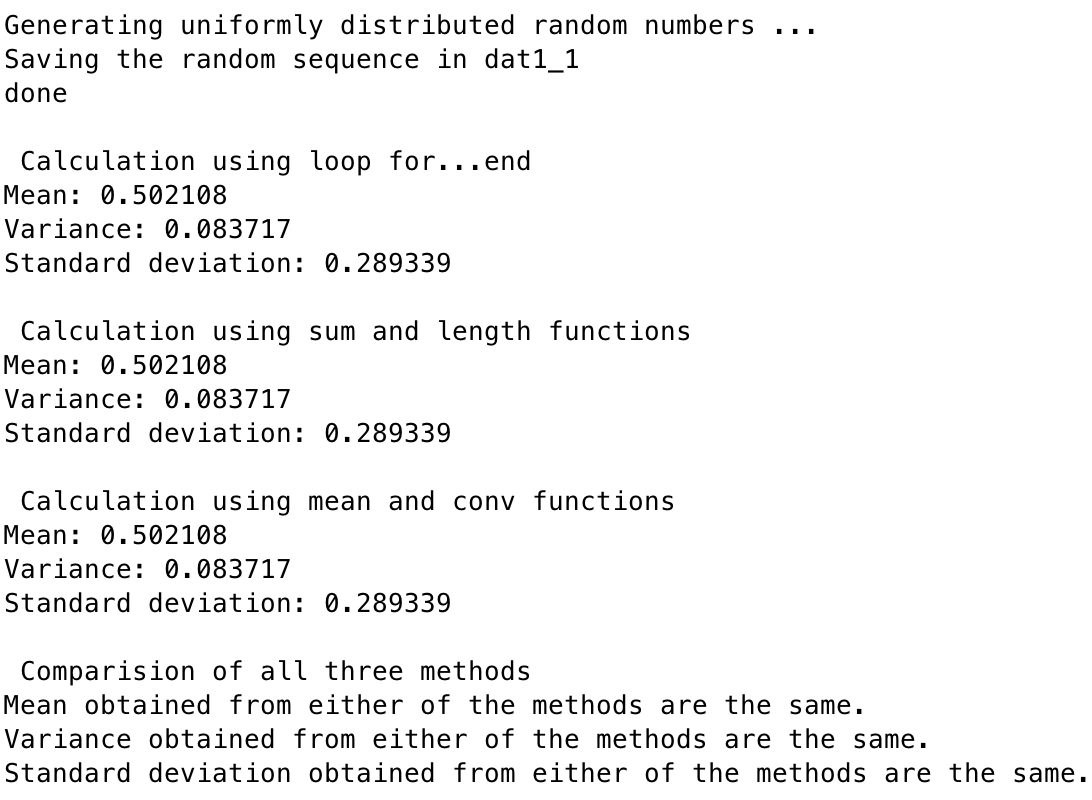
\includegraphics[scale=0.55]{ass1_2.png}}
\end{figure}
\noindent \textbf{Inference:} As observed from the above output, the mean, variance and the standard deviation calculated using the three different methods yields the same result.
%%%%%%%%%%%


\section{ Density function and histogram  } \label{ Density function and histogram }
\noindent \textbf{Task:} Write a function \texttt{density}, that estimates the density function of a random variable from a number of observations by applying the histogram function \texttt{hist}. Use the uniformly distributed random sequence from \texttt{dat1\_1}. Show the estimates as bar graph and as line graph. Compare the theoretical density function with the result by drawing the theoretical density also into the line graph figure. Repeat the experiment for 1000 standard normal distributed random numbers, where the initial value has to be set to 0. Save this random vector in \texttt{dat1\_2}.
(Note: The function \texttt{density} shall be applicable to any random sequences. Therefore take
into account the interrelationship between the scaling and the length of the random sequence and
the width of the interval.) 

\noindent \textbf{Solution:}
\noindent \texttt{density} function is written which allows the user to choose the number of \texttt{bins}. The uniform density function as well as the normal density function is estimated by using the function \texttt{hist}. Line graph of both theoretical and estimated values are plotted in-order to compare the two. 

\noindent \textbf{MATLAB code:}
\lstinputlisting{assignment1_2.m}

\noindent \textbf{Output:}
\noindent The estimated line and bar graph is plotted along with the theoretical graph for comparison. 
\begin{figure}[H]
\centering
{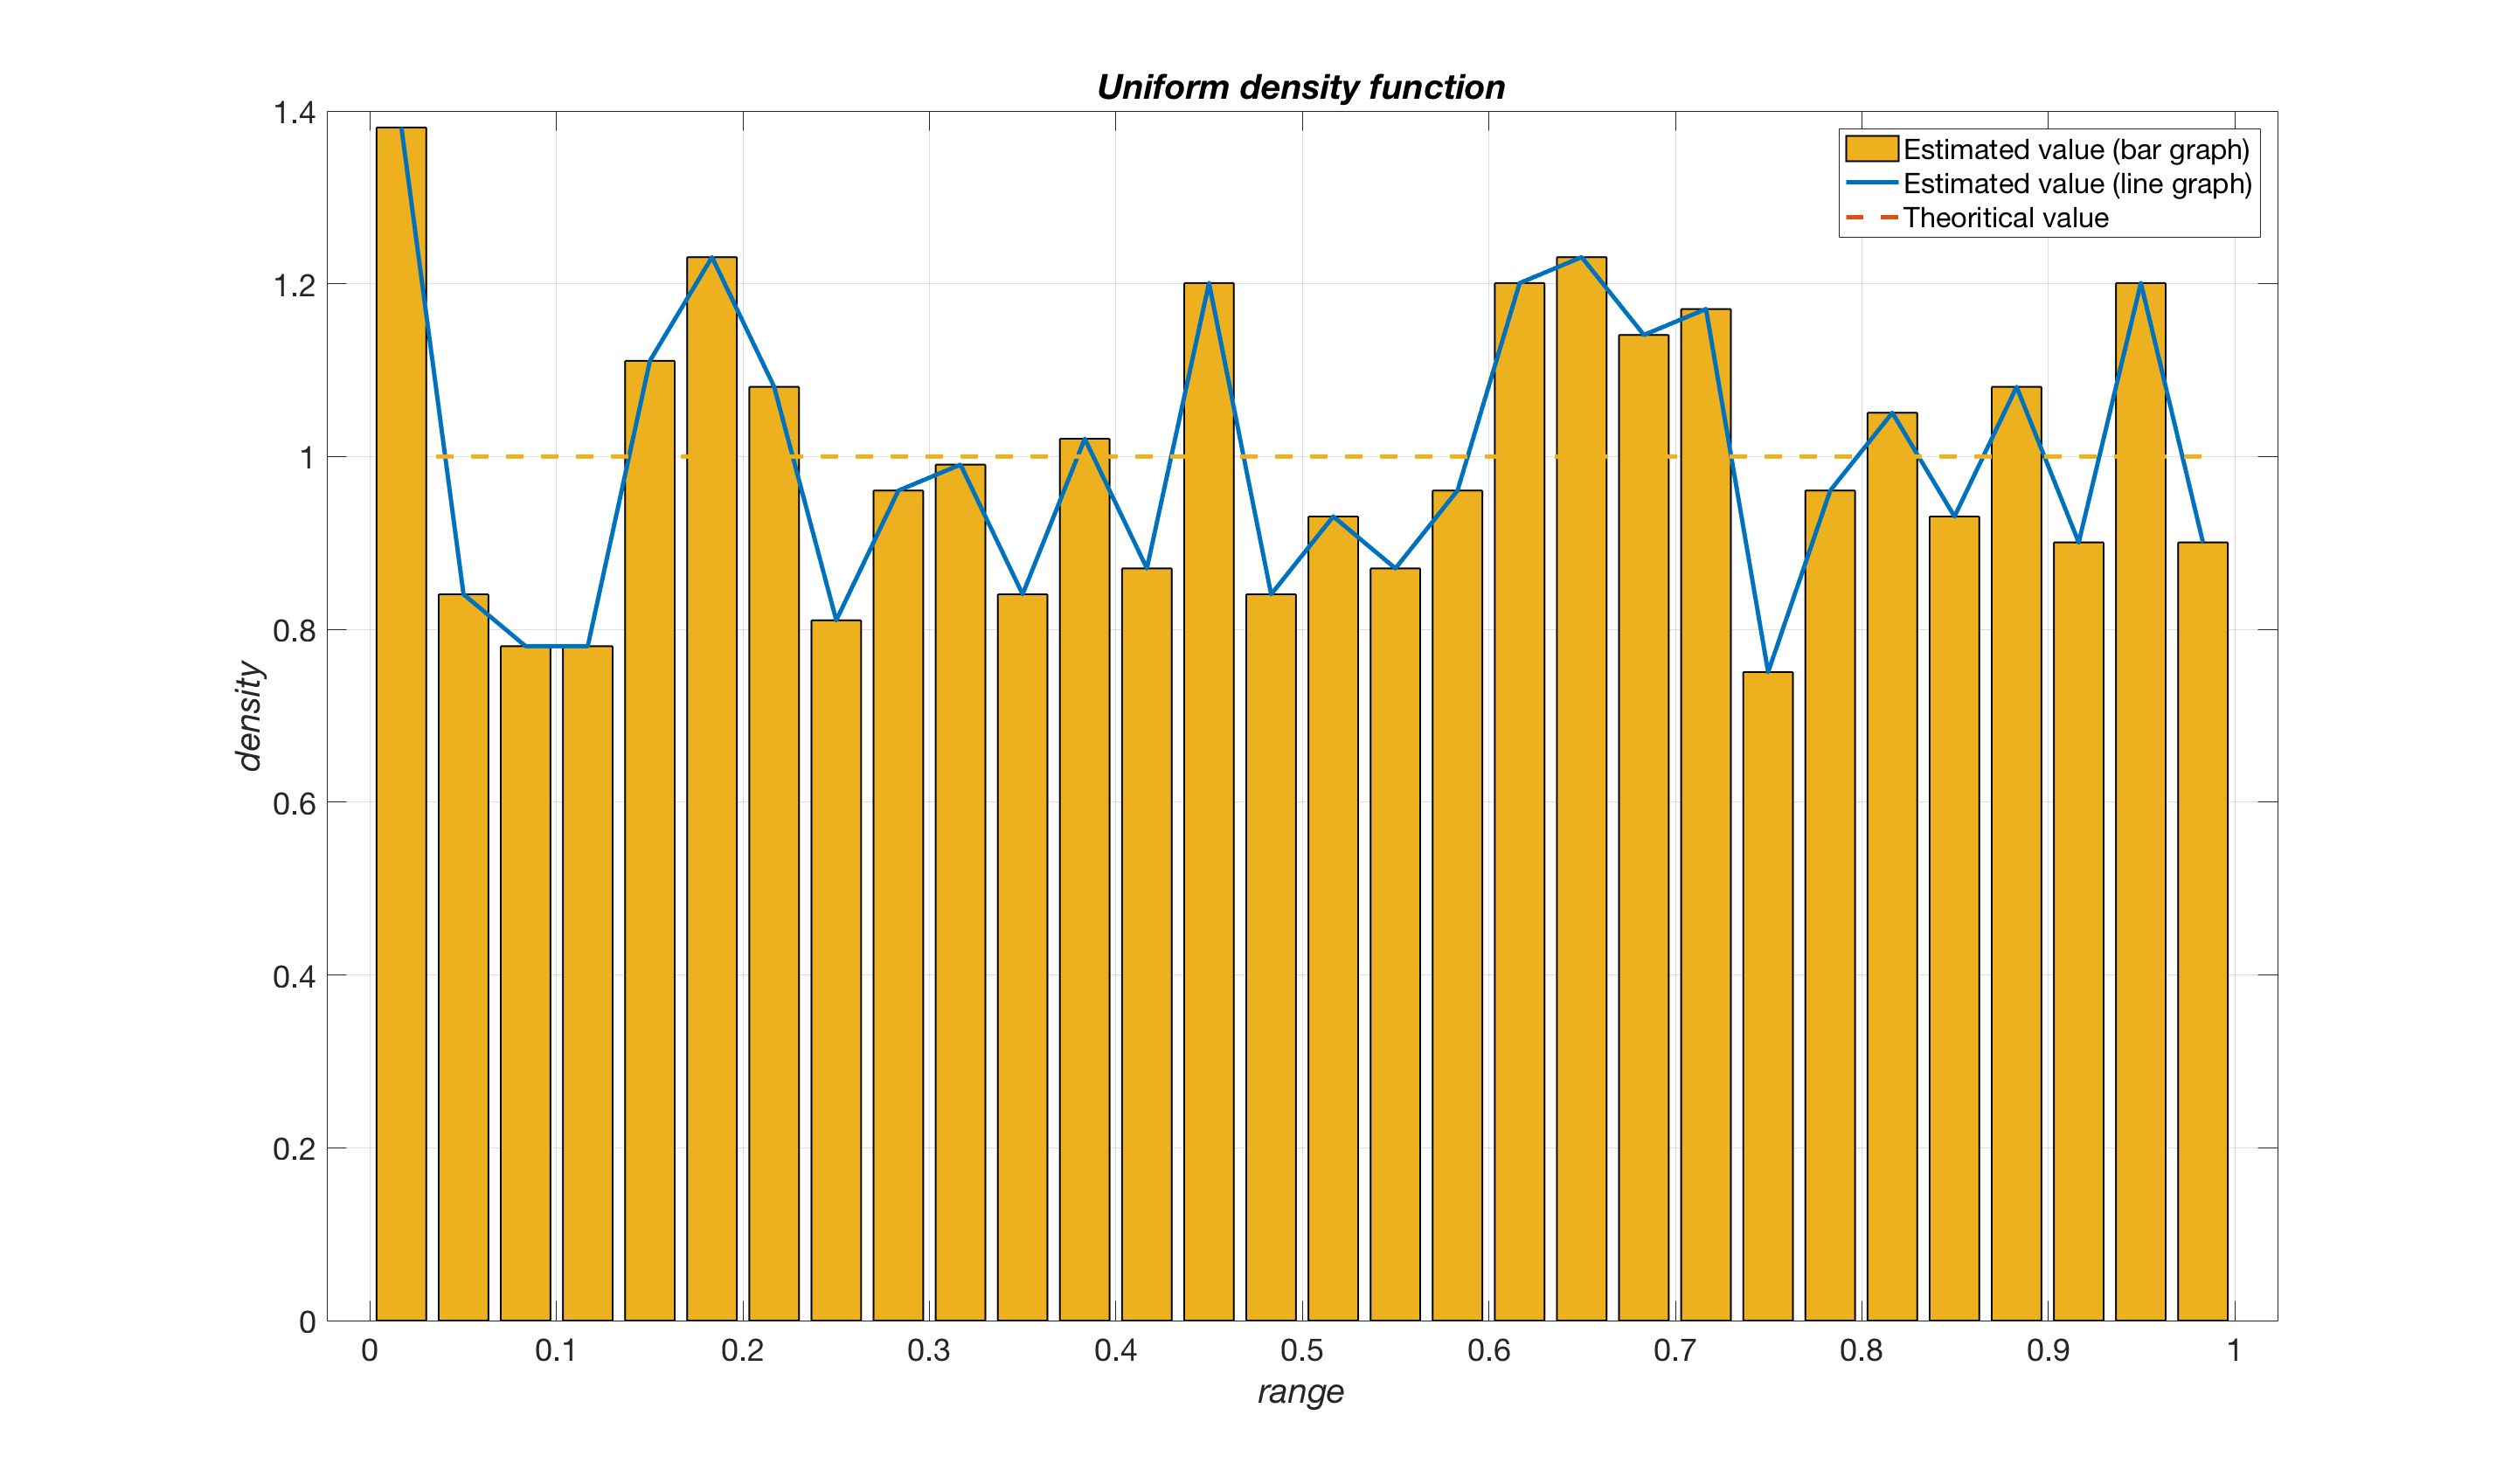
\includegraphics[scale=0.12]{ass2_1.png}}
\caption{Uniform density function}
\label{Uniform density function}
\end{figure}

\begin{figure}[H]
\centering
{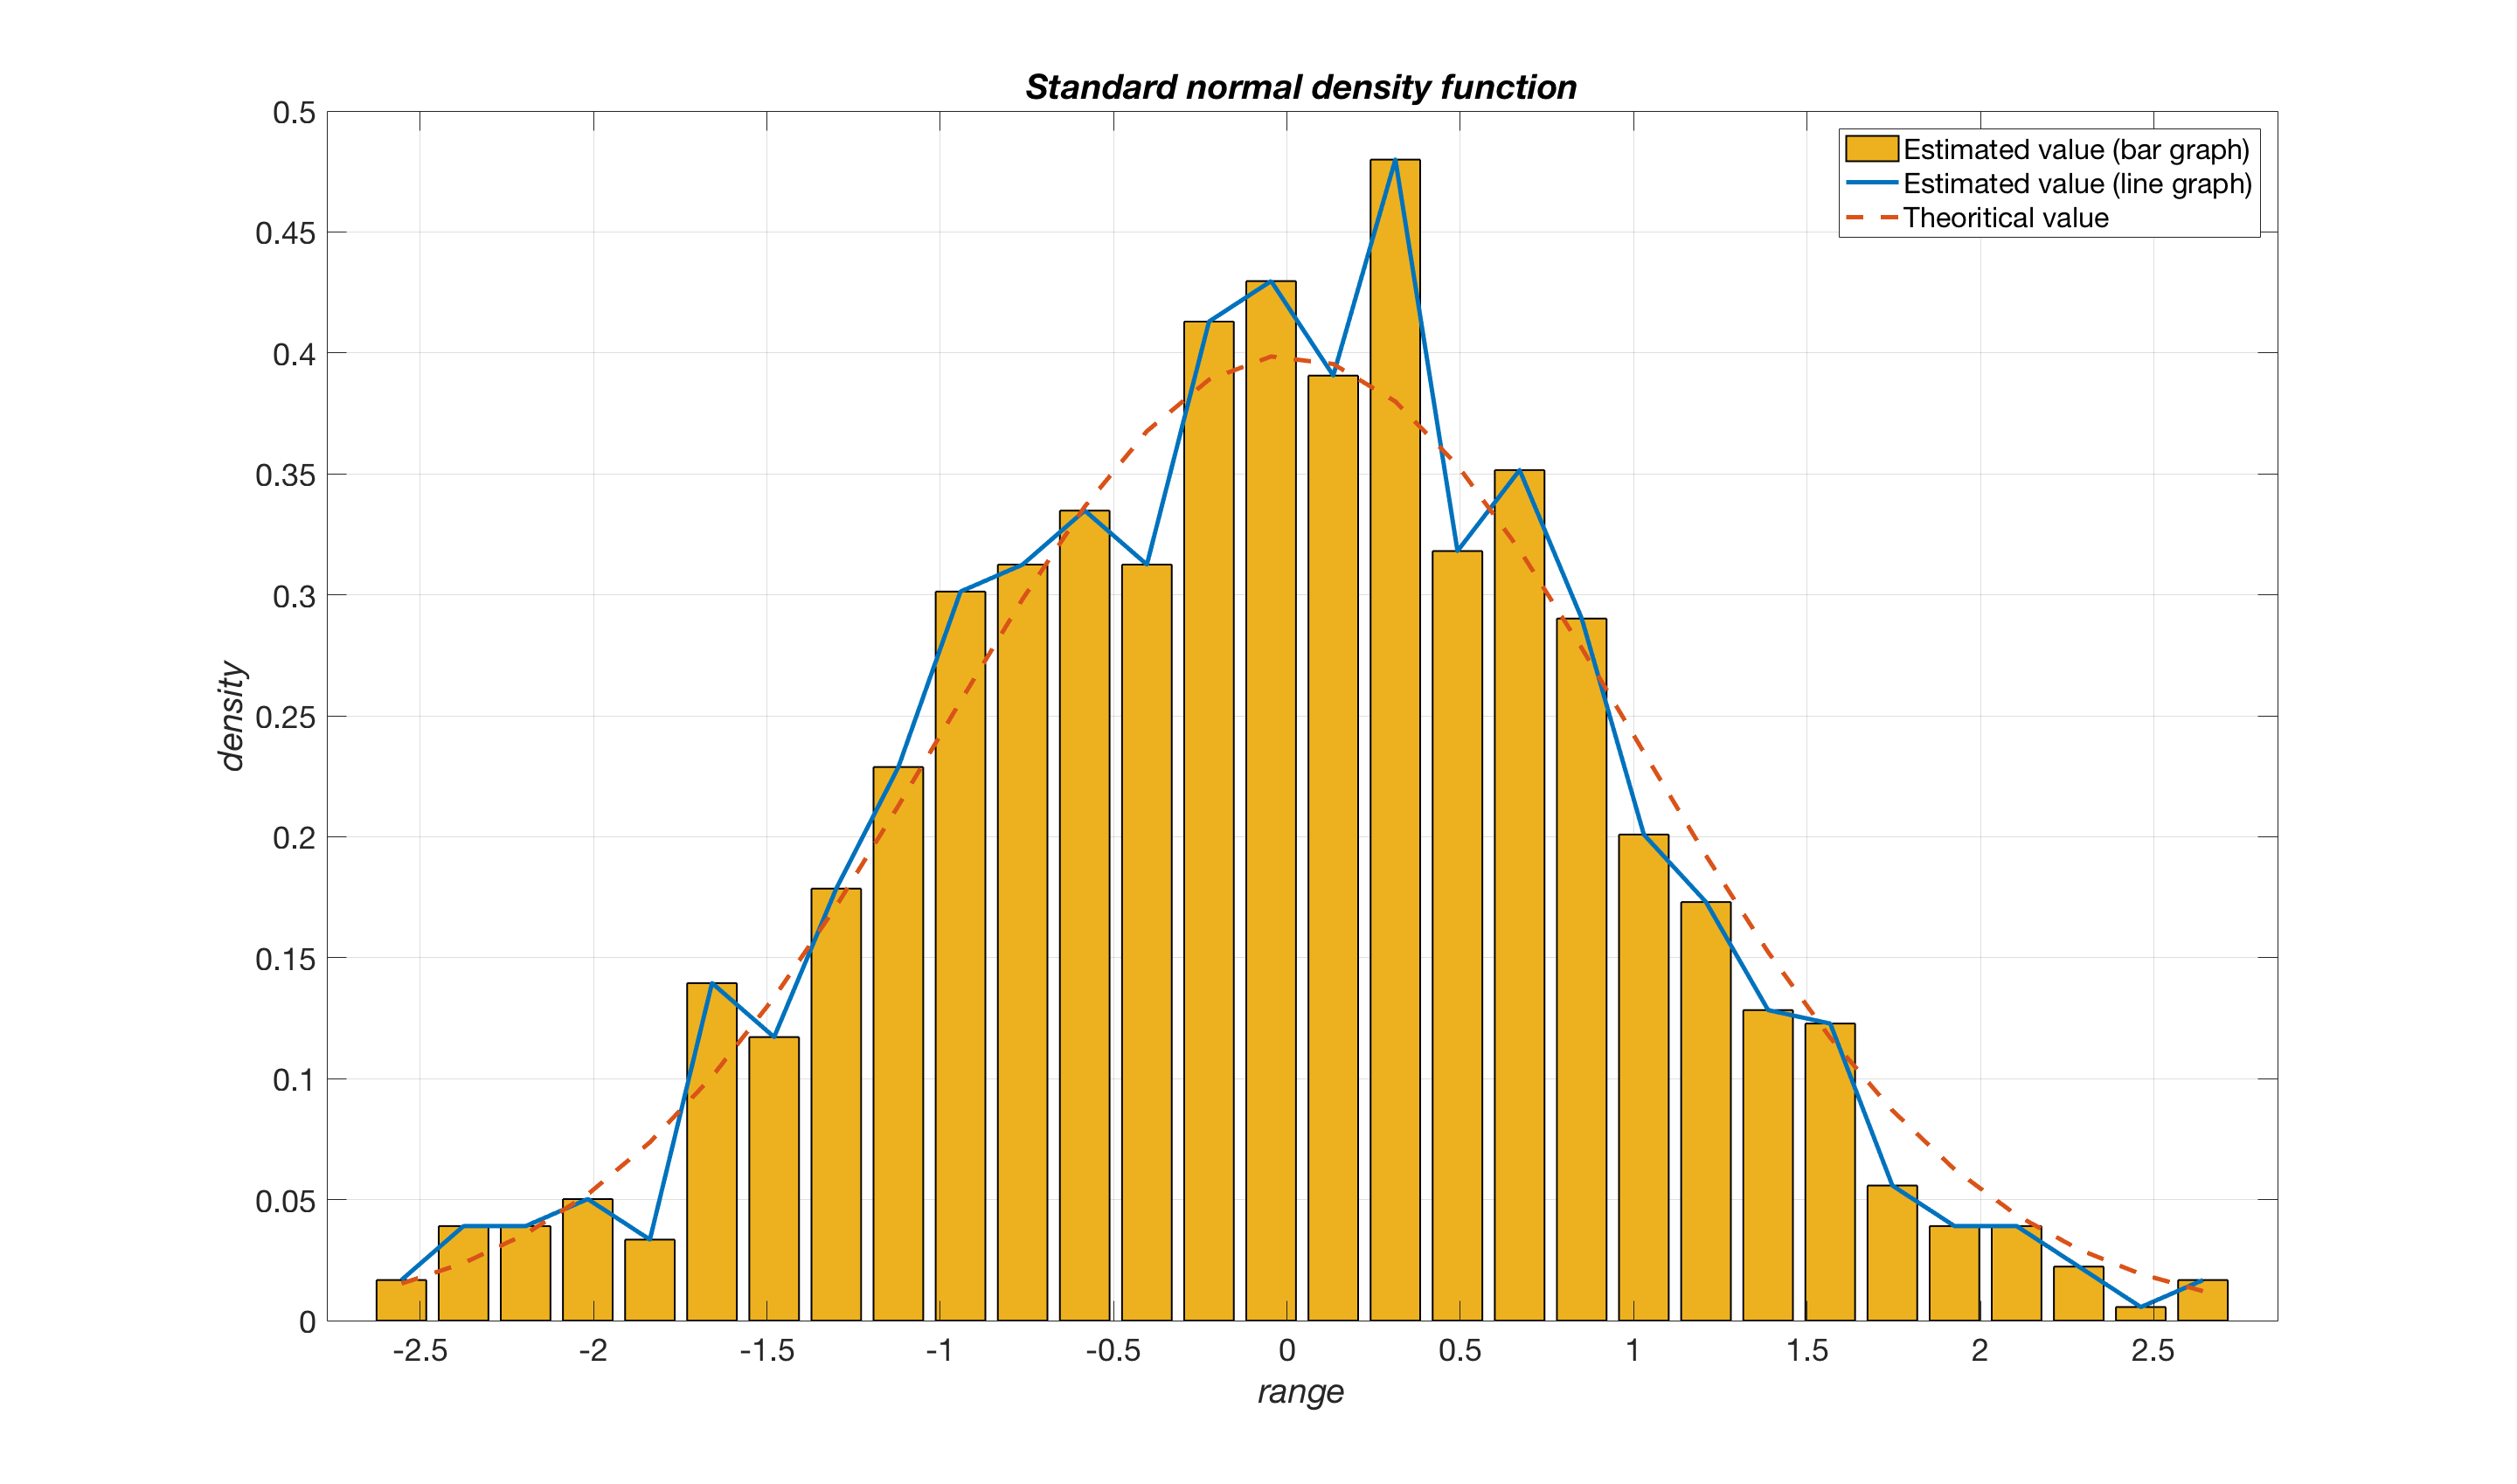
\includegraphics[scale=0.12]{ass2_2.png}}
\caption{Normal density function}
\label{Normal density function}
\end{figure}

\noindent The output of the code is shown below.
\begin{figure}[H]
\centering
{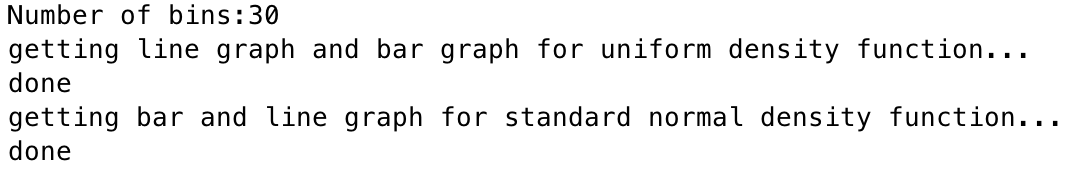
\includegraphics[scale=0.58]{ass2_3.png}}
\end{figure}

\noindent \textbf{Inference:} The values that are estimated using the histogram nearly coincide with the values estimated by the theoretical density function.
%%%%%%%%%%%%%%%


\section{ Distribution function and frequency  } \label{ Distribution function and frequency }
\noindent \textbf{Task:} Estimate the distribution function of the random sequences given in \texttt{dat1\_1} and \texttt{dat1\_2}. For this, generate with the MATLAB instruction \texttt{linspace} a rampe within the interval [0, 1] and use it for drawing the estimate. (Note: Sort the data.) 

\noindent \textbf{Solution:} the function \texttt{linespace} is used to generate a ramp within a given interval. we used this function to estimate the distribution function of random sequences that are stored in \texttt{dat\_1.mat} and texttt{dat\_2.mat}. The previously stored data needed to be sorted. In this case, we used the function \texttt{sort} to sort the data in increasing order.

\noindent \textbf{MATLAB code:}
\lstinputlisting{assignment1_3.m}


\noindent \textbf{Output:}
\noindent \texttt{dat\_1.mat} had the values for uniform distribution while \texttt{dat\_2.mat} consisted of values for the normal distribution. The plot of both the distribution is shown in Figure 2.4.
\begin{figure}[H]
\centering
{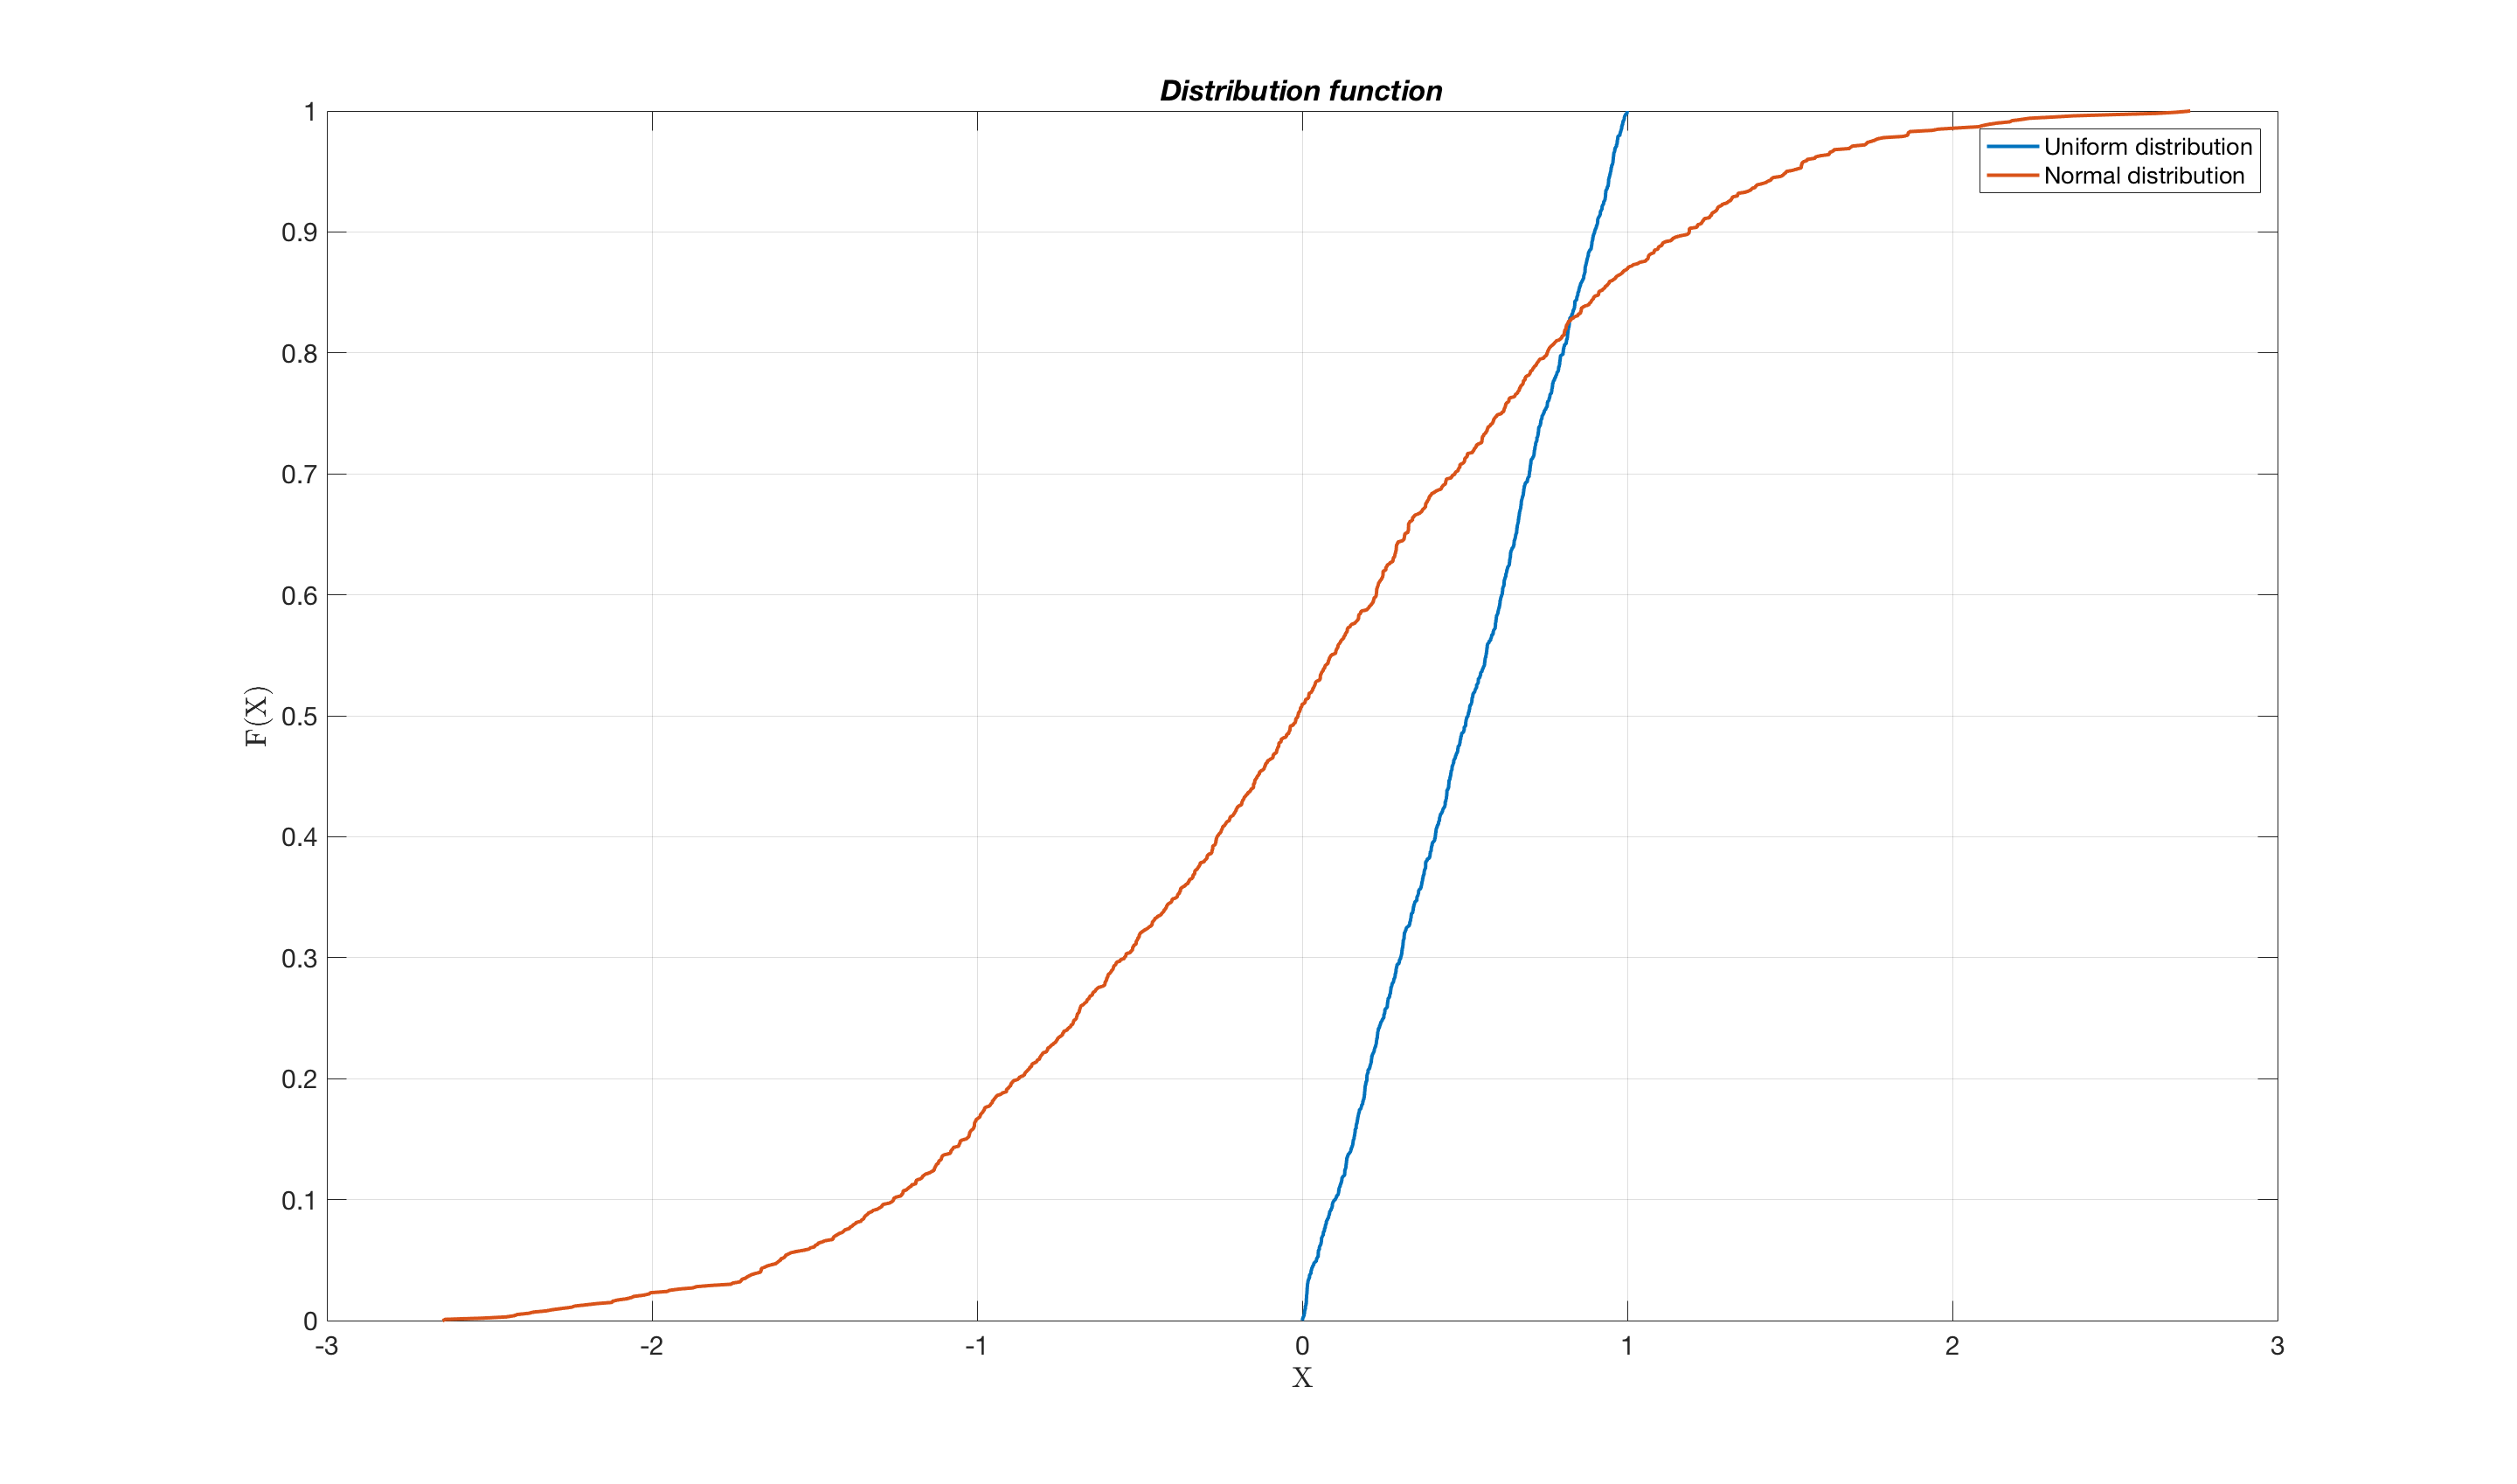
\includegraphics[scale=0.13]{ass3_1.png}}
\caption{Distribution function of random sequences}
\label{Distribution function of random sequences}
\end{figure}

\noindent In-order to get affirmation of the previously stored data, \texttt{exist} function was used to check the presence of the files and the number of random numbers were printed.
\begin{figure}[H]
\centering
{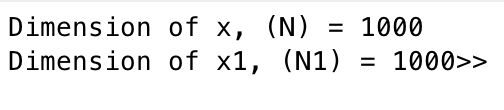
\includegraphics[scale=0.68]{ass3_2.png}}
\end{figure}

\noindent \textbf{Inference:} The plotted graph shows that the previously stored data is correct.


%%%%%%%%


\section{ Generation of a bivariate normal distribution  } \label{ Generation of a bivariate normal distribution  }
\noindent \textbf{Task:} Set the initial value of \texttt{randn} to 0. Generate through \texttt{z1=randn(1000,2)} a matrix of normal distributed random numbers. Multiply \texttt{z1} from the right with the matrix \texttt{D = [1 .5; 0 .5]}, thus \texttt{z2 = z1 * D.} Separate the result through \texttt{x = z2(:,1)} and \texttt{y = z2(:,2)} into two vectors and add 1.5 to each element of \texttt{x} and 0.5 to each element of y. Store the vectors by using the MATLAB instruction \texttt{save dat1\_3 x y.}

\noindent \textbf{Solution:} The \texttt{dat1\_3} was saved by following the instructions step-by-step as mentioned in the task. To check for validation, \texttt{whos} function was used and the variable names were printed.

\noindent \textbf{MATLAB code:}
\lstinputlisting{assignment1_4.m}

\noindent \textbf{Output:} The output after execution of the code is shown below.
\begin{figure}[H]
\centering
{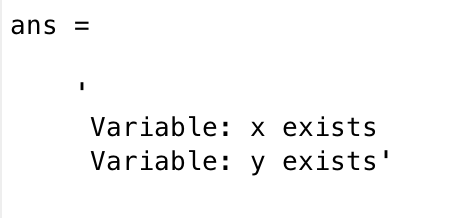
\includegraphics[scale=0.58]{ass4_1.png}}
\end{figure}

\noindent \textbf{Inference:} Variable \texttt{x} and variable \texttt{y} exists. Thus we can say that we have successfully implemented the mentioned task.
%%%%%%%%%%%


\section{ Bivariate normal distribution } \label{ Bivariate normal distribution}
\noindent \textbf{Task:} Load \texttt{dat1\_3} that includes the two vectors \texttt{x} and \texttt{y} of length 1000 as samples of the two bivariate normally distributed random variables \texttt{X} and \texttt{Y}. Estimate for this dataset $\mu_x$, $\mu_y$, $\sigma_x^2$, $\sigma_y^2$  and $\rho$ by using the sample cross- and covariance function. Calculate the bivariate density function $f_{x,y}(x,y)$ with the estimated parameters and display it as a 3dimensional and a level curve graphic. (Note: Use the MATLAB-functions mesh and contour.) 
 
 \noindent \textbf{Solution:} First, a function \texttt{getParameters} was written in-order to get the values of $\mu_x$, $\mu_y$, $\sigma_x^2$, $\sigma_y^2$  and $\rho$. Later, these values were required to calculate the Bivariate normal distribution. The 3D view of the distribution was plotted using \texttt{mesh}.
 
 \noindent \textbf{MATLAB code:}
\lstinputlisting{assignment1_5.m}

 \noindent \textbf{Output:}
 \noindent Figure 2.5 is the result from the execution of the code. $\rho$ found by using the formula for these data sets was 0.6529. Hence it is a little more flattened in the perpendicular direction as compared to when $\rho$ is 0. At 0, the graph is perfectly symmetric bell shaped and parallel to the horizontal line.
\begin{figure}[H]
\centering
{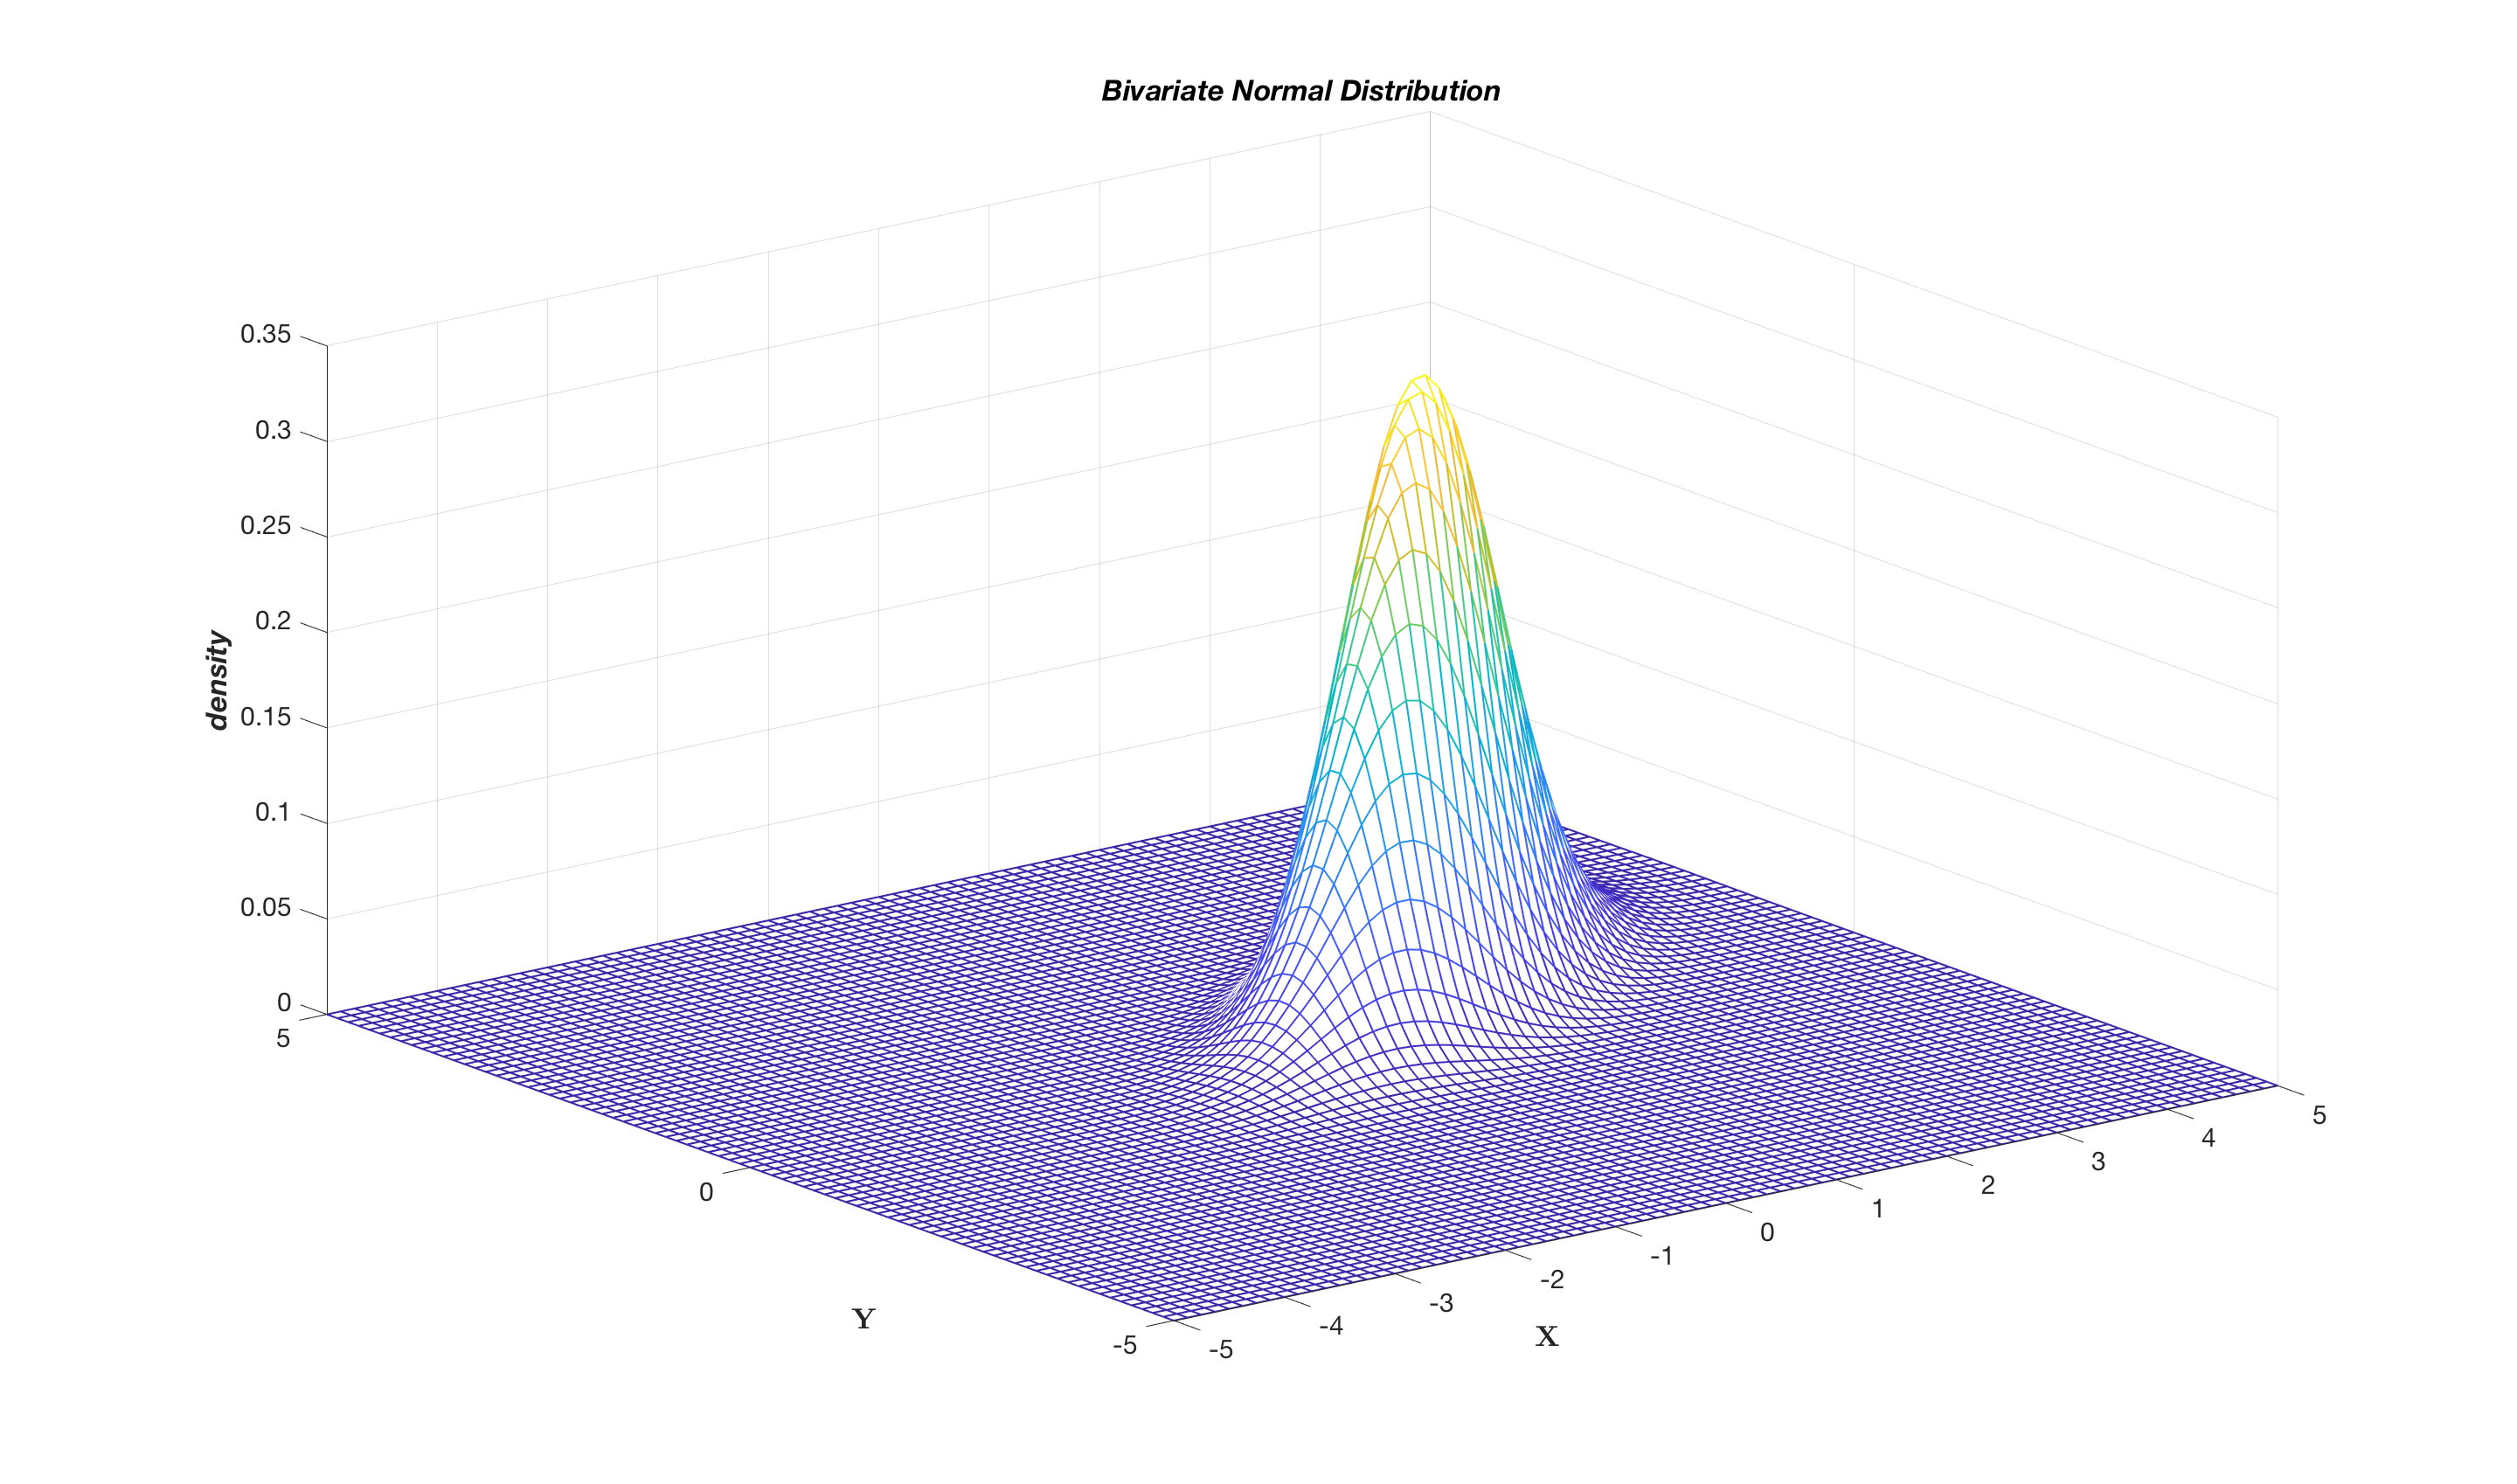
\includegraphics[scale=0.13]{ass5_1.png}}
\caption{3 dimensional view of Bivariate normal distribution}
\label{3 dimensional view of Bivariate normal distribution}
\end{figure}

\begin{figure}[H]
\centering
{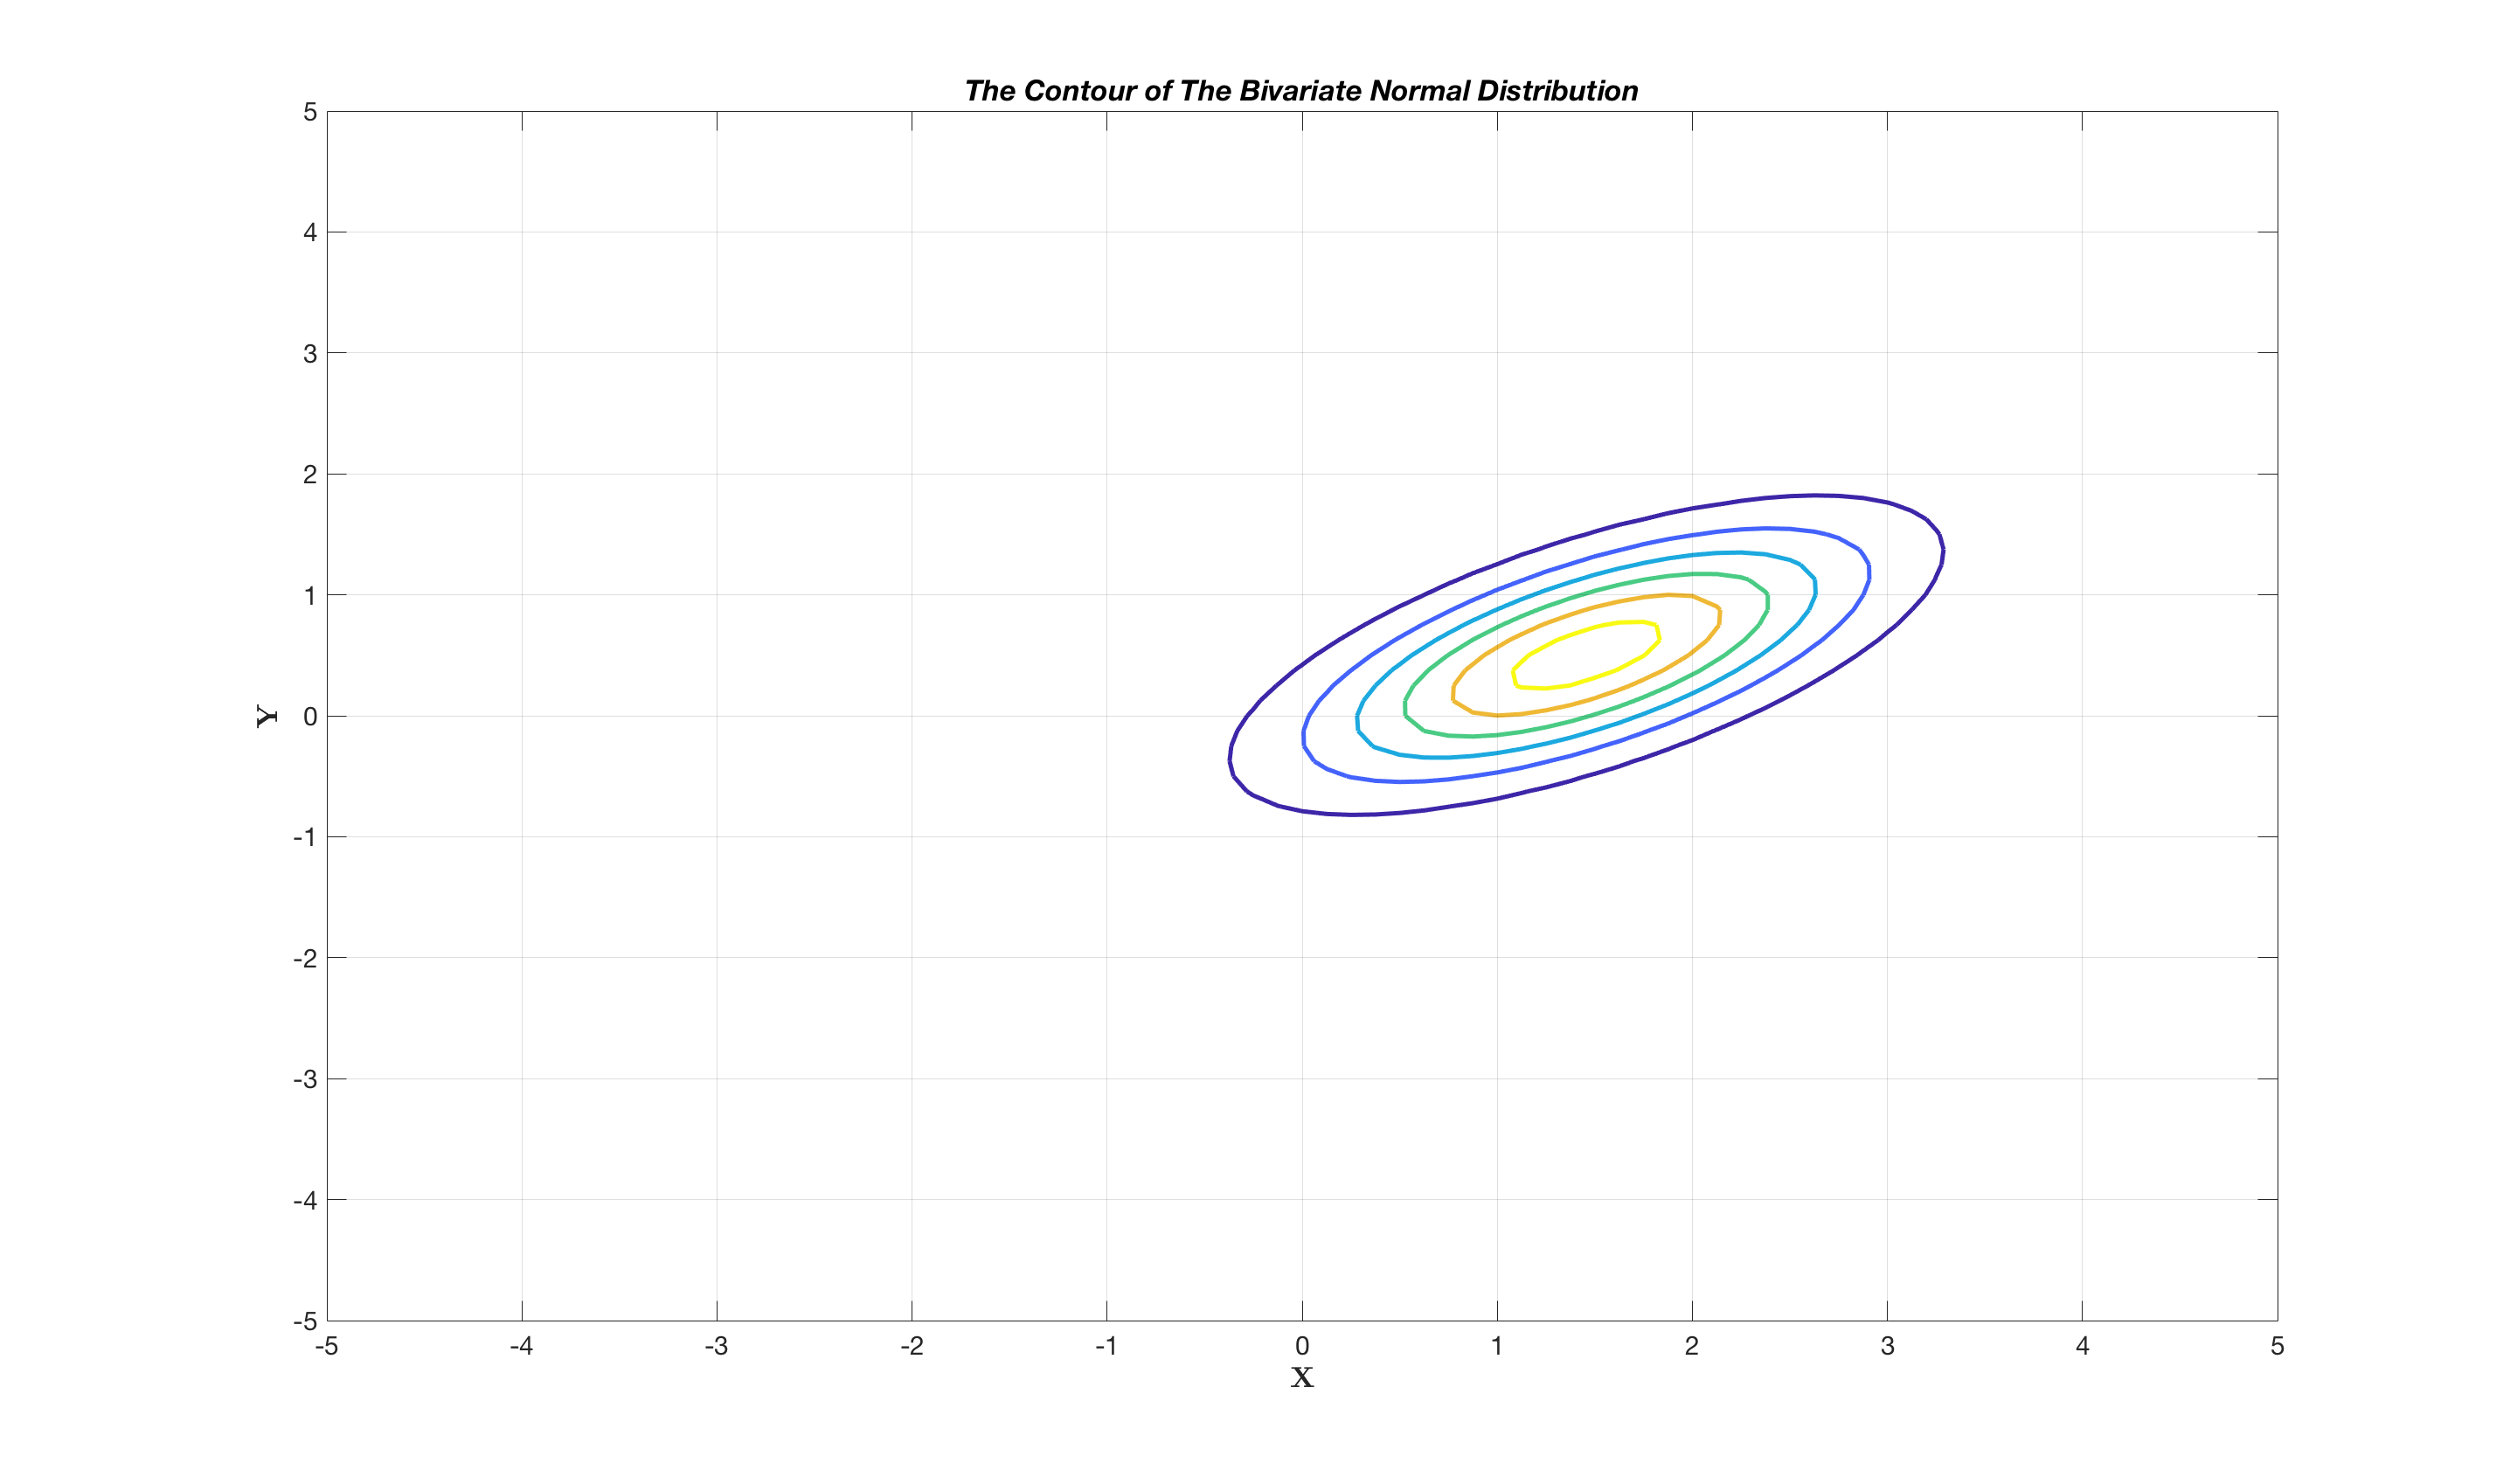
\includegraphics[scale=0.13]{ass5_2.png}}
\caption{Contour of the Bivariate normal distribution}
\label{Contour of the Bivariate normal distribution}
\end{figure}

\noindent \textbf{Inference:} As $\rho$ increases, that bell-shaped curve becomes flattened on the 45 degree line. At $\rho$ equals 0.65, we can see that the curve extends out towards minus 3 and plus 3 and becomes flattened in the perpendicular direction.
%%%%%%
\section{ Monte-Carlo-Method for approximation of $\pi$ }  \label{Monte-Carlo-Method }
\noindent \textbf{Task:} Generate two on the interval [0, 1] uniformly distributed random sequences \texttt{x} and \texttt{y} of length 1000. The initial value has to be set to 0 again. How many points lie within the unit circle? Estimate therewith the constant $\pi$ .

\noindent \textbf{Solution:} First, \texttt{x} and \texttt{y} in the range of [0,1] are created using \texttt{rand}. Further, the code is written to find the number of points within a circle of radius 1. We have allowed the users to choose the length of the uniformly distributed random sequence. We aim to find the relationship between the actual value of $\pi$ and the length of the sequence chosen.

\noindent \textbf{MATLAB code:} 
\lstinputlisting{assignment1_6.m}

\noindent \textbf{Output:} The output of the code is shown below. We considered the length of the sequence to be 1000 as mentioned in the task.
\begin{figure}[H]
\centering
{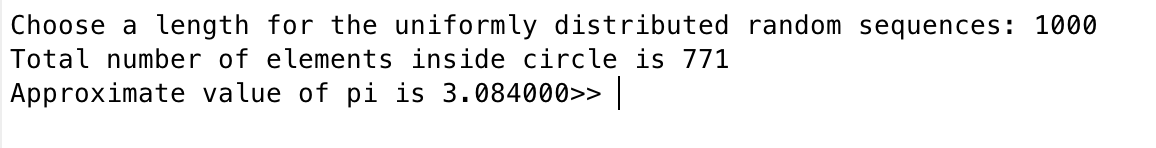
\includegraphics[scale=0.58]{ass6_1.png}}
\end{figure}
\noindent We further wrote another program to find how the length of the sequence affects the value of $\pi$. 
\lstinputlisting{assignment1_6_additional.m}
\noindent We notice from Figure 2.7 that as the length of the sequence increases, we get a better approximation of $\pi$.
\begin{figure}[H]
\centering
{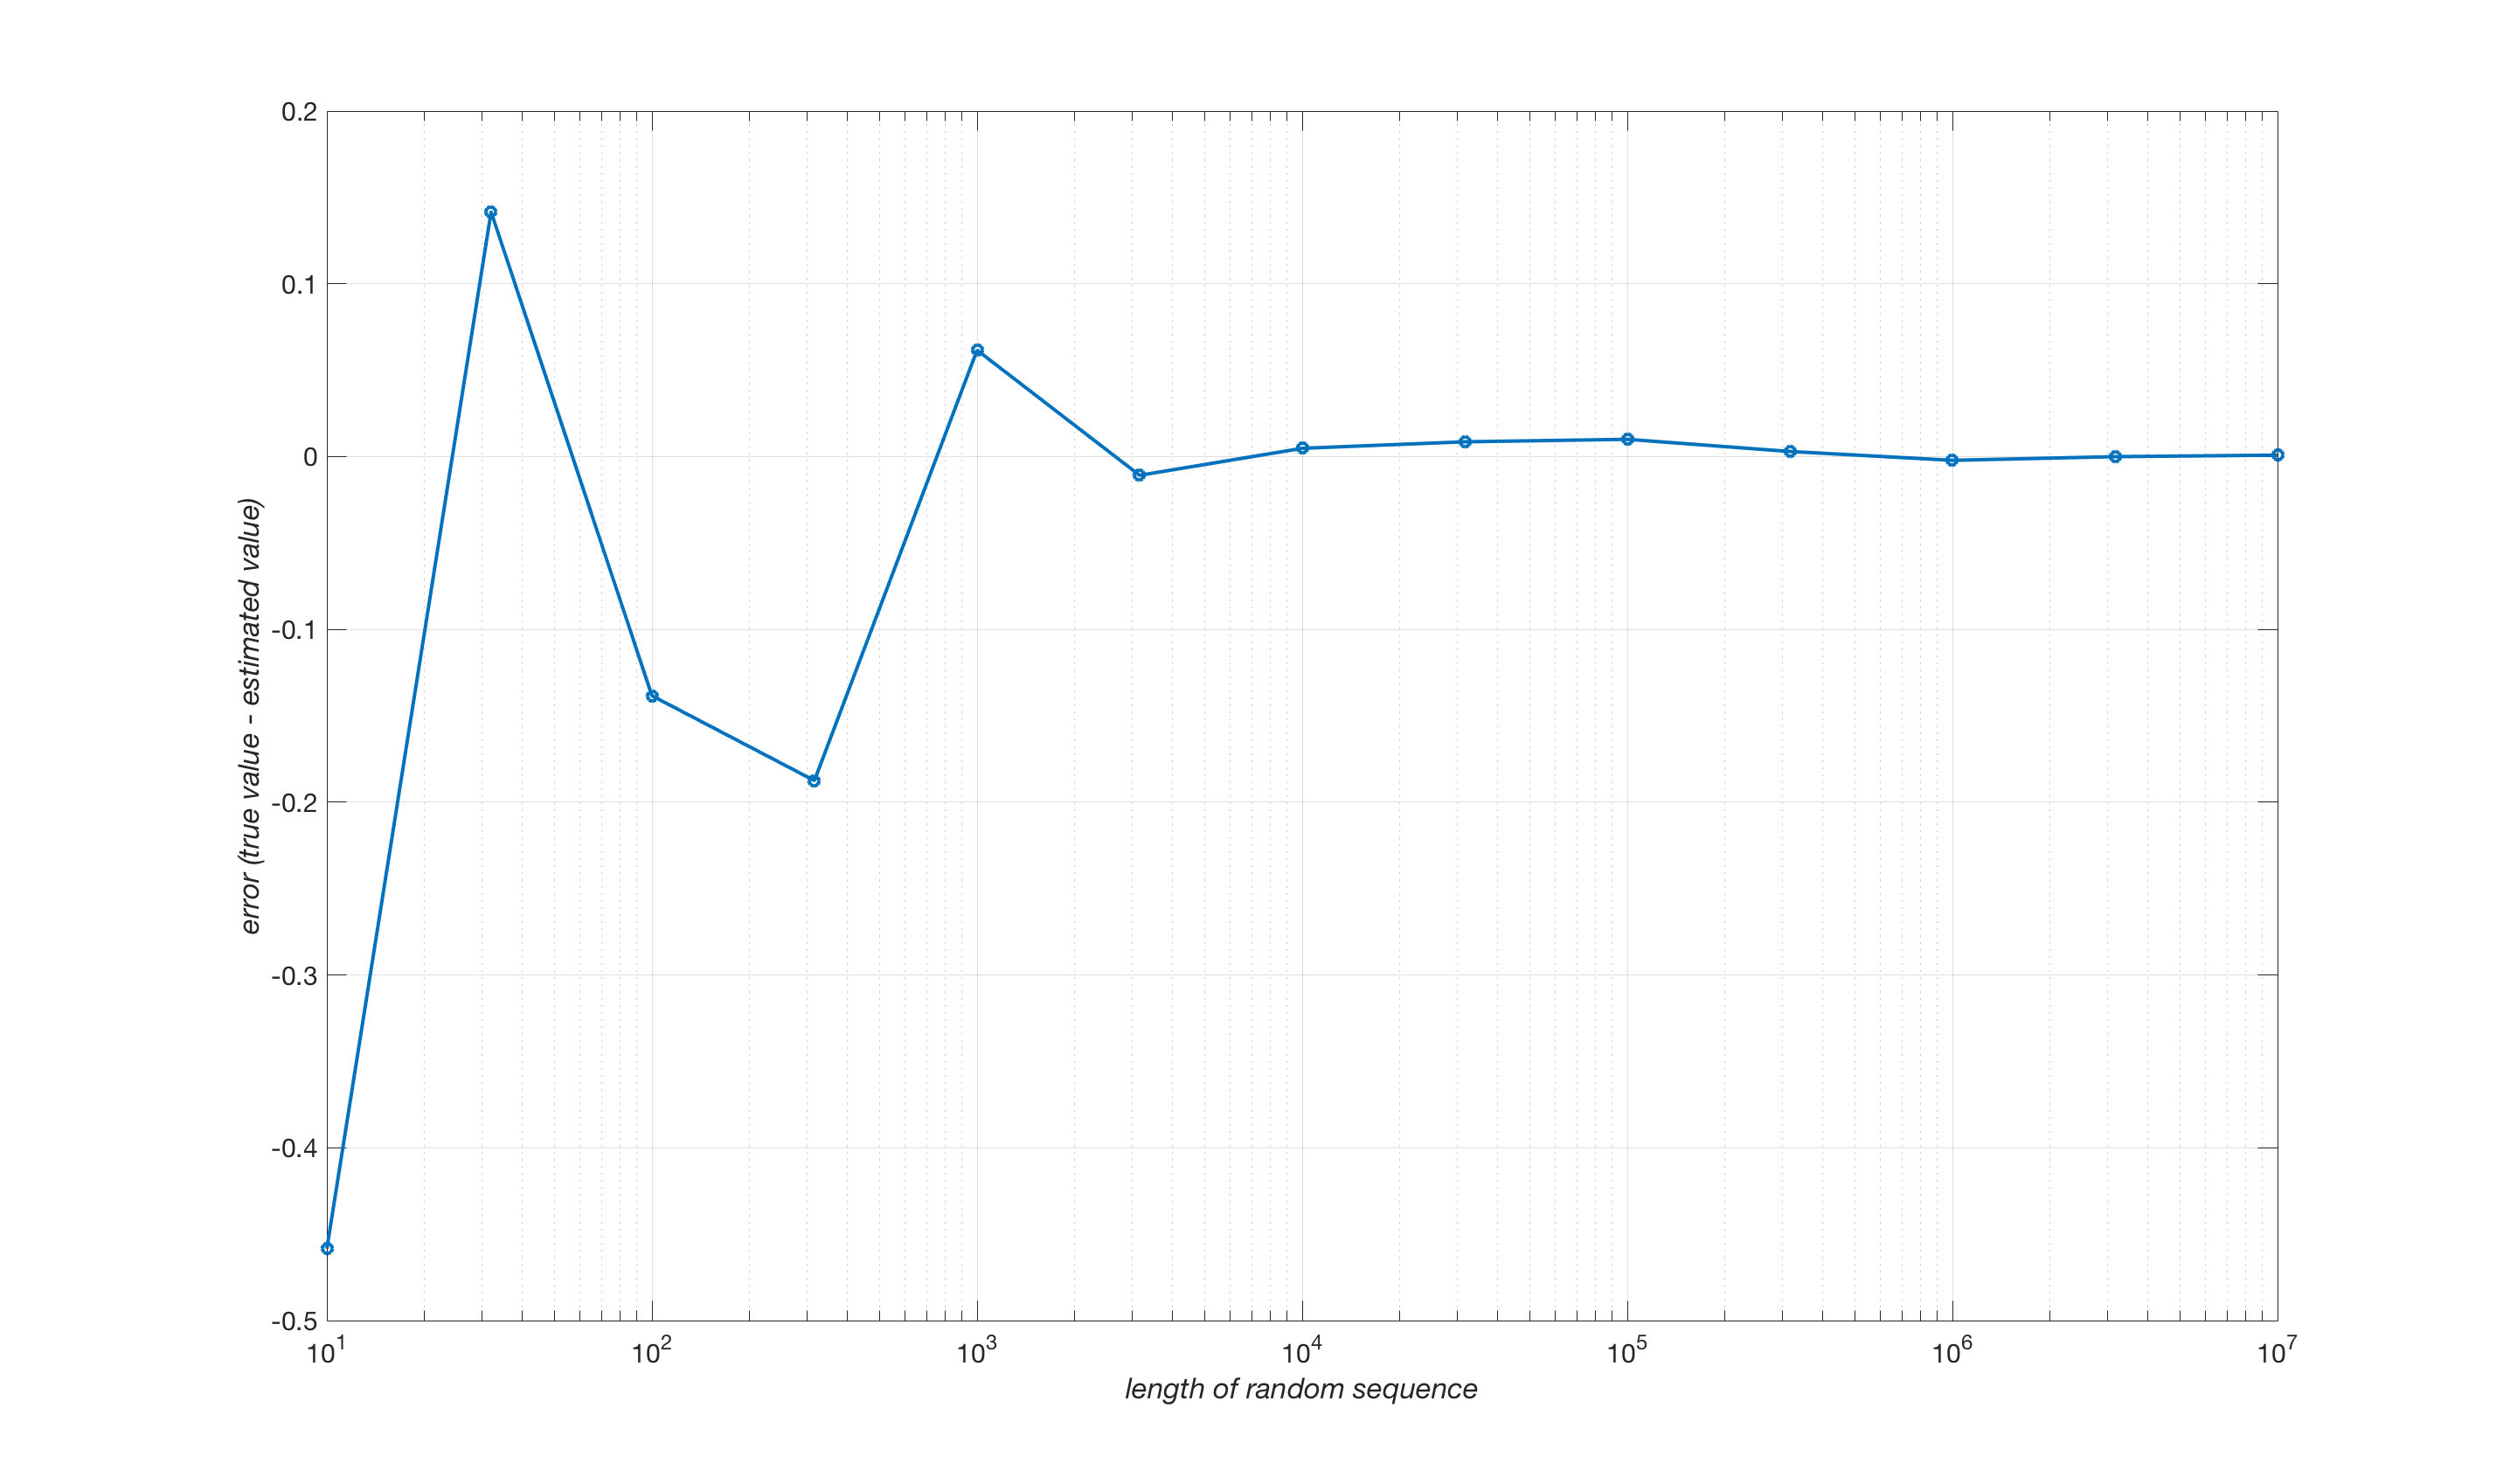
\includegraphics[scale=0.13]{ass6_2.png}}
\caption{Length of random sequence versus the error value}
\label{Length of random sequence versus the error value}
\end{figure}

\noindent \textbf{Inference:} From Figure 2.7, it is proved that as we increase the length of the sequence from 1000 to 100000 (100 times), we have a much better estimation of $\pi$.
